\documentclass[./SoftwareEngineering.tex]{subfiles}


\section{Mô hình thiết kế}

\begin{figure}[!htb]
	\centering
	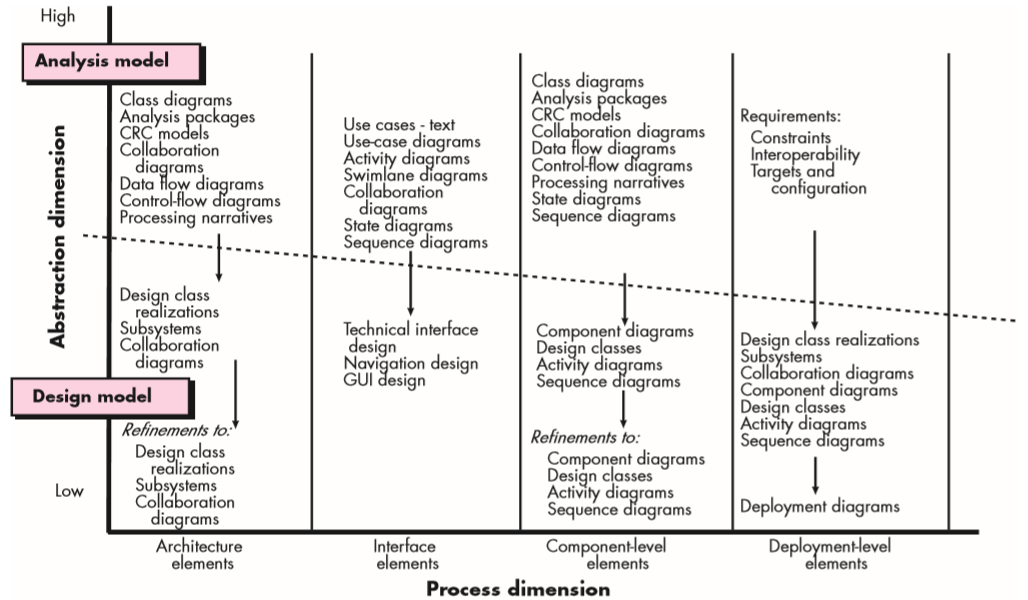
\includegraphics[width=\textwidth]{figure_8_4.png}
	\caption{Chiều của mô hình thiết kế}
	\label{fig:fig8_4}
\end{figure}

Mô hình thiết kế có thể được quan sát theo 2 chiều khác nhau như được thể hiện trong \autoref{fig:fig8_4}.  \textit{Chiều quá trình} (process dimension) biểu thị sự tiến hóa của mô hình thiết kế trong khi các task được thực hiện như là một phần trong các quá trình của phần mềm. \textit{Chiều trừu tượng} (abstraction dimension) đại diện cho mức độ chi tiết khi mỗi yếu tố của mô hình phân tích được biến đổi thành một thiết kế tương ứng và cải thiện một cách lặp đi lặp lại. Theo \autoref{fig:fig8_4}, đường nét đứt biểu thị ranh giới giữa mô hình phân tích và thiết kế. Trong một vài trường hợp, việc phân biệt rõ mô hình phân tích và thiết kế là khả thi. Trong vài trường hợp khác, mô hình phân tích dần trộn lẫn với mô hình thiết kế nên đường phân biệt sẽ ít rõ ràng hơn.  


Các yếu tố của mô hình thiết kế có sử dụng nhiều biểu đồ UML mà cũng được sử dụng trong mô hình phân tích. Điểm khác biệt là các biểu đồ này được cải thiện và bổ sung như là một phần của thiết kế; bổ sung các chi tiết cụ thể về việc thực thi được cung cấp, cùng với cấu trúc kiến trúc và phong cách, các thành phần trú ngụ bên trong kiến trúc, giao diện giữa các thành phần và với thế giới bên ngoài đều được nhấn mạnh. 

Tuy nhiên, các yếu tố của mô hình biểu thị dọc theo trục hoành không phải lúc nào cũng được phát triển theo hướng tuần tự. Trong hầu hết các trường hợp, thiết kế kiến trúc sơ bộ sẽ đặt nền móng và được theo sau bởi thiết kế giao diện và thiết kế mức độ thành phần, hai việc mà thường sẽ xảy ra song song. Mô hình triển khai sẽ bị hoãn đến khi thiết kế được hoàn thiện. Người đọc có thể áp dụng design pattern vào bất kỳ thời điểm nào trong quá trình thiết kế. Các mẫu này cho phép ta áp dụng những kiến thức về thiết kế với các vấn đề thuộc từng phạm vi cụ thể mà đã được giải quyết.


\subsection{Các yếu tố của thiết kế dữ liệu}
Cũng giống như các hoạt động thiết kế phần mềm khác, thiết kế dữ liệu (đôi khi được nhắc đến như là \iindex{kiến trúc dữ liệu}) tạo ra một mô hình của dữ liệu và/hoặc thông tin mà được thể hiện ở mức độ trừu tượng cao (dữ liệu dưới góc nhìn của khách hàng/người dùng). Mô hình dữ liệu này sau đó được tinh chỉnh dần dần thành các đại diện cụ thể của việc thực thi mà có thể được xử lý bởi hệ thống dựa trên máy tính. Trong nhiều ứng dụng, kiến trúc của dữ liệu sẽ có những ảnh hưởng sâu sắc đến kiến trúc của phần mềm xử lý nó. 

Cấu trúc của dữ liệu vẫn luôn là một phần quan trọng của thiết kế phần mềm. Ở cấp độ bộ phận của chương trình, thiết kế của dữ liệu và các thuật toán được yêu cầu để điều khiển chúng là thiết yếu với việc chế tạo một ứng dụng chất lượng cao. Ở cấp độ ứng dụng, bản dịch của một mẫu dữ liệu (xuất phát như một phần của kỹ thuật yêu cầu) vào cơ sở dữ liệu là mấu chốt để đạt được các mục tiêu kinh doanh của một hệ thống. Ở cấp độ kinh doanh, việc thu thập thông tin được lưu trữ trong các cơ sở dữ liệu khác nhau và được sắp xếp lại thành “kho dữ liệu” cho phép khai thác dữ liệu hoặc khám phá các kiến thức có thể ảnh hưởng đến sự thành công của chính việc kinh doanh. Trong mọi trường hợp, thiết kế dữ liệu đều đóng một vai trò quan trọng.

\subsection{Các yếu tố của thiết kế kiến trúc}
Thiết kế kiến trúc cho phần mềm tương đương với sơ đồ mặt bằng của một ngôi nhà. Sơ đồ mặt bằng mô tả bố cục tổng thể của các phòng; kích thước, hình dạng và mối quan hệ của chúng với nhau; và các cửa ra vào và cửa sổ cho phép di chuyển vào và ra khỏi phòng. Sơ đồ mặt bằng cho chúng ta một cái nhìn tổng thể về ngôi nhà.Tương tự, các yếu tố thiết kế kiến trúc cho chúng ta cái nhìn tổng thể về phần mềm. 

Mô hình kiến trúc \cite{Sha96} được lấy từ ba nguồn: (1) thông tin về miền ứng dụng cho phần mềm sẽ được xây dựng; (2) các yếu tố mô hình được yêu cầu cụ thể như biểu đồ luồng dữ liệu hoặc các lớp phân tích, mối quan hệ và sự hợp tác của chúng cho vấn đề hiện tại; và (3) sự sẵn có của các kiểu kiến trúc và các mẫu. 

Yếu tố thiết kế kiến trúc thường được mô tả như một tập hợp các hệ thống con được kết nối với nhau, thường được lấy từ các gói phân tích trong mô hình yêu cầu. Mỗi hệ thống con có thể có kiến trúc riêng của nó (ví dụ: giao diện người dùng có thể được cấu trúc theo kiểu kiến trúc có sẵn cho giao diện người dùng). Những kỹ thuật lấy các yếu tố cụ thể của mô hình kiến trúc được trình bày trong chương tiếp theo của tài liệu chính thức.  


\subsection{Thiết kế giao diện}
Thiết kế giao diện cho phần mềm tương tự như một tập hợp các bản vẽ chi tiết (và thông số kỹ thuật) cho các cửa ra vào, cửa sổ và các tiện ích bên ngoài của một ngôi nhà. Những bản vẽ này mô tả kích thước và hình dạng của cửa ra vào và cửa sổ, cách thức vận hành, cách thức các liên kết tiện ích (ví dụ như nước, điện, ga, điện thoại) dẫn vào nhà và được phân phối giữa các phòng được mô tả trong sơ đồ mặt bằng. Chúng cho ta biết chuông cửa được đặt ở đâu, có sử dụng máy liên lạc để thông báo sự hiện diện của khách truy cập hay không và cách cài đặt hệ thống bảo mật. Về bản chất, các bản vẽ chi tiết (và thông số kỹ thuật) cho cửa ra vào, cửa sổ và các tiện ích bên ngoài cho chúng ta biết cách mà mọi thứ và thông tin được đưa vào và ra khỏi nhà và giữa các phòng thuộc sơ đồ mặt bằng. Các yếu tố thiết kế giao diện cho phần mềm mô tả thông tin vào và ra khỏi hệ thống và cách nó được truyền đạt giữa các thành phần được xác định là một phần của kiến trúc. 

Có ba yếu tố quan trọng của thiết kế giao diện: (1) giao diện người dùng (UI); (2) giao diện bên ngoài với các hệ thống, thiết bị, mạng, nhà sản xuất hoặc người tiêu dùng; và (3) giao diện nội bộ giữa các thành phần thiết kế khác nhau. Các yếu tố thiết kế giao diện này cho phép phần mềm giao tiếp với bên ngoài và cho phép giao tiếp và hợp tác nội bộ giữa các thành phần tạo nên kiến trúc phần mềm. 

Thiết kế UI (ngày càng được gọi là \iindex{thiết kế khả dụng}) là một phần chính của kỹ thuật phần mềm và được giải thích chi tiết trong một chương khác của tài liệu chính thức. Thiết kế khả dụng kết hợp các yếu tố thẩm mỹ (vd: bố cục, màu sắc, đồ họa, cơ chế tương tác), các yếu tố công thái học (vd: bố trí và sắp xếp thông tin , ẩn dụ, UI điều hướng) và các yếu tố kỹ thuật (ví dụ: mẫu UI, các thành phần có thể tái sử dụng). Nói chung, UI là một hệ thống con độc nhất trong kiến trúc ứng dụng tổng thể. 

Việc thiết kế các giao diện bên ngoài đòi hỏi thông tin dứt khoát về thực thể mà thông tin đó được gửi đến hoặc nhận. Trong mọi trường hợp, thông tin này phải được thu thập trong quá trình yêu cầu kỹ thuật và được xác minh khi thiết kế giao diện bắt đầu. Thiết kế giao diện bên ngoài nên kết hợp kiểm tra lỗi và (nếu cần) các tính năng bảo mật thích hợp. 
Thiết kế của các giao diện bên trong được liên kết chặt chẽ với thiết kế tầng thành phần. Thiết kế của các lớp phân tích đại diện cho tất cả các hoạt động và các kế hoạch cần thiết để cho phép giao tiếp và hợp tác giữa các hoạt động trong các lớp khác nhau. Mỗi thông điệp phải được thiết kế để phù hợp với việc truyền thông tin cần thiết và các yêu cầu chức năng cụ thể của hoạt động đã được yêu cầu. Nếu cách tiếp cận cổ điển đầu vào - tiến trình - đầu ra để thiết kế được chọn, giao diện của từng thành phần phần mềm được thiết kế dựa trên các biểu diễn luồng dữ liệu và chức năng được mô tả trong tường thuật xử lý. 


Trong một số trường hợp, một giao diện được mô hình hóa tương tự với một lớp. Trong UML, một giao diện được định nghĩa theo cách sau \cite{Gro03}: “Giao diện là chỉ định cho các hoạt động [công khai] có thể nhìn thấy bên ngoài của một lớp, thành phần hoặc phân loại khác (bao gồm cả các hệ thống con) mà không có đặc điểm kỹ thuật của cấu trúc bên trong”. Nói một cách đơn giản hơn, giao diện là một tập hợp các hoạt động mô tả một phần hành vi của một lớp và cung cấp quyền truy cập vào các hoạt động này. 


\begin{figure}[!htb]
	\centering
	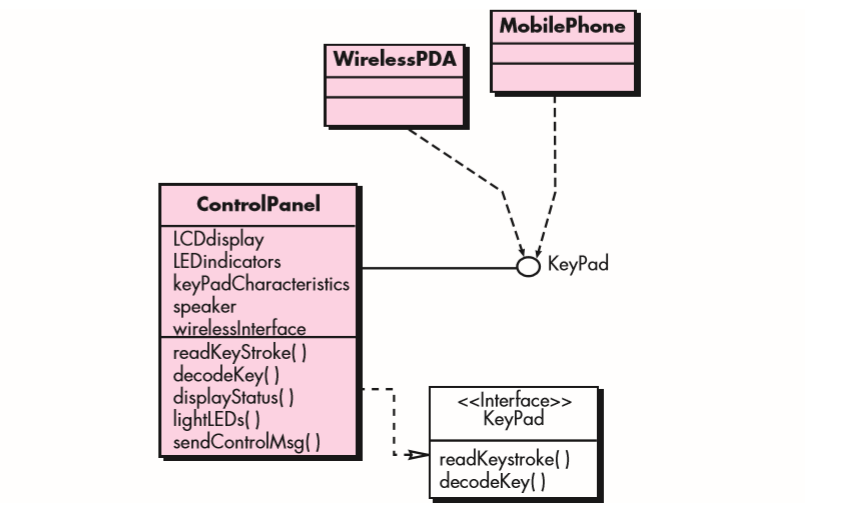
\includegraphics[width=\textwidth]{figure_8_5.png}
	\caption{Mô tả giao diện cho ControlPanel}
	\label{fig:fig8_5}
\end{figure}


Ví dụ: chức năng bảo mật \textit{SafeHome} sử dụng bảng điều khiển cho phép chủ nhà kiểm soát các khía cạnh nhất định của chức năng bảo mật. Trong phiên bản nâng cao của hệ thống, các chức năng của bảng điều khiển có thể được thực hiện thông qua một thiết bị không dây PDA hoặc điện thoại di động.

Lớp \textbf{ControlPanel} \autoref{fig:fig8_5} cung cấp hành vi liên quan tới bàn phím, do đó, nó phải thực hiện các hoạt động \textit{readKeyStroke()} và \textit{decodeKey()}. Nếu các hoạt động này được cung cấp cho các lớp khác (trong trường hợp này là \textbf{WirelessPDA} và \textbf{MobilePhone}), sẽ rất hữu ích khi xác định giao diện như trong hình. Giao diện này, được đặt tên là \textbf{KeyPad}, được hiển thị dưới dạng khuôn mẫu <<interface>> hoặc dưới dạng một vòng tròn nhỏ, được gắn nhãn kết nối với lớp bằng một đường kẻ. Giao diện được xác định không có thuộc tính và tập hợp các thao tác cần thiết để đạt được hành vi của bàn phím.
\subsection{Thiết kế các yếu tố ở cấp thành phần}
au quá trình thiết kế kiến trúc, ta đã xác định được một kiến trúc hoàn chỉnh các thành phần của phần mềm. Nhưng cấu trúc dữ liệu và chi tiết của từng thành phần không được biểu diễn rõ ràng. Vì vậy, thiết kế cấp thành phần chính là bước xác định cấu trúc dữ liệu, thuật toán, đặc điểm giao diện và cơ chế truyền thông được phân bổ cho từng thành phần.

Bản thiết kế cấp thành phần của phần mềm như là một bản thiết kế chi tiết về mỗi phòng của một ngôi nhà. Bản vẽ đó miêu tả đầy đủ về vị trí đường dây, ống nước mỗi phòng, vị trí của ổ điện và công tắc, bồn tắm, phòng vệ sinh , tủ quần áo,…. Chúng cũng miêu tả phần nền móng, phần khung xương và mọi chi tiết khác có liên quan trong căn phòng.

Thiết kế cấp thành phần miêu tả đầy đủ những chi tiết bên trong từng thành phần. Để đạt được điều đó, thiết kế cấp thành phần khai báo những cấu trúc dữ liệu cho tất cả các đối tượng dữ liệu địa phương và thuật toán chi tiết cho tất cả những tiến trình xảy ra ở thành phần và interface cho phép truy cập với tất cả những hoạt động của thành phần.

\begin{figure}[!htb]
	\centering
	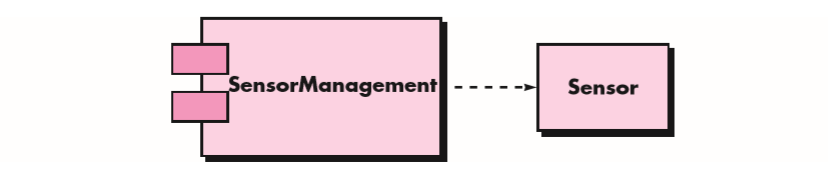
\includegraphics[width=\textwidth]{figure_8_6.png}
	\caption{Sơ đồ thành phần UML}
	\label{fig:fig8_6}
\end{figure}

Trong trường hợp phần mềm hướng tới đối tượng, một sơ đồ thành phần UML được biểu diễn \autoref{fig:fig8_5} Trong hình này là  một thành phần có tên là \textbf{SensorManagement}( Quản lý cảm biến) ( một phần trong các chức năng của SafeHome). Mũi tên nét đứt nối với class có tên là \textbf{Sensor} được kế thừa từ đó.

\textbf{Thành phần SensorManagement} có tất cả những hàm liên quan đến class \textbf{Sensor}( cảm biến của \textit{SafeHome}) bao gồm cả việc giám sát và cấu hình chung. Thiết kế chi tiết của các thành phần sẽ được kế thừa qua các lớp trừu tượng.  Những logic của component có thể được trình bày bằng một sơ đồ UML.

Luồng điều khiển của thành phần có thể được thể hiện bằng mã giả hoặc một sơ đồ khác. Thuật toán thì sẽ được tuân theo những quy tắc được thiết lập trước, cấu trúc dữ liệu thì dựa trên bản chất của đối tượng và được mô hình bằng mã giả hoặc ngôn ngữ lập trình.



\subsection{Thiết kế sơ đồ triển khai}
Sơ đồ triển khai các thành phần biểu thị cách mà các chức năng và các hệ thống con được phân bổ trong môi trường mà phần mềm đang chạy. Ví dụ, các thành phần của \textit{SafeHome} được cài đặt hoạt động trong 3 môi trường: -một PC tại nhà; - bảng điều khiển \textit{SafeHome}, và một server đặt tại CPI( cung cấp khả năng truy cập hệ thống qua internet).

\begin{figure}[!htb]
	\centering
	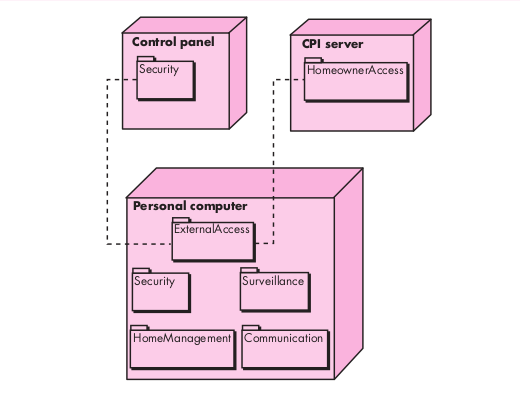
\includegraphics[width=\textwidth]{figure_8_7.png}
	\caption{Sơ đồ triển khai UML}
	\label{fig:fig8_7}
\end{figure}


 Trong\autoref{fig:fig8_7} là ba môi trường điện toán được biểu thị ( thực chất sẽ nhiều hơn nếu tính đến cảm biến, camera,vv). Mỗi chức năng được đặt trong một môi trường chỉ định. Ví dụ, máy tính cá nhân sẽ bao gồm các chương trình con như security( bảo mật), giám sát, quản lý nhà, và tính năng liên lạc. Ngoài ra,  còn có chương trình quản lý các truy cập từ nguồn bên ngoài. Mỗi một chương trình con/ hệ thống con ấy sẽ được xây dựng dựa theo thành phần mà nó thực hiện.
 
Sơ đồ\autoref{fig:fig8_7} chỉ là \textit{dạng mô tả}, nó bao quát các phần của các môi trường điện toán và không chỉ ra rõ ràng, chi tiết. Ví dụ, “máy tính cá nhân” chỉ chung chung, nó có thể chạy hệ điều hành Mac, Window hay linux. Những thông tin đó( cấu hình cụ thể, phần cứng,..) sẽ được tìm hiểu ở giai đoạn sau của thiết kế hoặc khi bắt đầu xây dựng.
